\documentclass{article}
\usepackage{graphicx}
\usepackage{fancyhdr}
\usepackage{listings}

\let\<\textless
\let\>\textgreater

\graphicspath{ {images/} }
\pagestyle{fancy}
\fancyhf{}
\rhead{Proyecto \#2}
\rfoot{P\'agina \thepage}

\begin{document}
\begin{titlepage}
  \centering
  {\scshape\LARGE Instituto Tecnol\'ogico de Costa Rica \par}
  \vspace{1cm}
  {\scshape\Large Redes\par}
  {\scshape\Large Proyecto \#2 - IT\par}
  \vspace{1.5cm}
  {\Large\itshape Allan Rojas\par}
  {\Large\itshape Sa\'ul Zamora\par}
  \vfill
  profesor\par
  Kevin Moraga \textsc{}

  \vfill

% Bottom of the page
  % {\large \today\par}
\end{titlepage}

\section{Introducci\'on}
El presente proyecto pretende ser una gu\'ia para la instalaci\'on de una red de servicios segura. Para ello, se hace uso exhaustivo de la tecnolog\'ia de virtualizaci\'on con el fin de instalar todo el ambiente en una sola m\'aquina f\'isica. Se crear\'a una LAN virtual que ser\'a la que ofrece los diversos servicios a trav\'es de un gateway que la conectar\'a con una WAN, desde la cual se consumir\'an los servicios ofrecidos por la LAN.

\section{Ambiente de trabajo}
\begin{itemize}
  \item Windows 10
  \item WIndows Server 2012
  \item CentOS 7
  \item OpenSUSE 13.2
  \item Debian 7
  \item Debian 8
  \item OpenBSD 5.8
  \item Docker
  \item FreeBSD 10
  \item FreePBX
  \item Ubuntu 18 LTS
\end{itemize}

\section{Dise\~no}

\section{Instalaci\'on de servicios}
\subsection{Lanzamiento de instancias en OpenStack}
NOTA: para que los siguientes pasos apliquen, es requerido tener configurado con anterioridad el proyecto, redes, usuarios, sabores e im\'agenes disponibles.

\begin{enumerate}
  \item Ingresar al panel de OpenStack.
  \item Abrir el men\'u de instancias a la izquierda.
  \item Hacer clic en el bot\'on de "Launch Instance".
  \begin{figure}[!h]
    \centering
      
\includegraphics{images/instances-1.png}
    \label{fig:graph}
  \end{figure}
  \item En "Instance Name" ingresar el nombre que recibir\'a la instancia.
  \item En la opci\'on de "Boot Source" escoger "Boot from image (creates a new volume)" y escoger la imagen deseada.
  \item En la opci\'on de "Image Name" seleccionar la imagen deseada.
  \item En la opci\'on de "Device Size (GB)" ingresar el tama\~no deseado para el almacenamiento en disco de la instancia (las distintas im\'agenes tienen distintos requerimientos de almacenamiento).
  \item En la pesta\~na de de "Access \& Seciruty" seleccionar el keypair deseado para accesar la instancia. (Pasos para la creaci\'on del keypair ser\'an mostrados m\'as adelante).
  \item En la pesta\~na de "Networking" agregar la red default.
  \item En la pesta\~na de "Post-creation" se pueden agregar reglas personalizadas.
  \item Clic en "Launch" para lanzar la instancia.
\end{enumerate}

\subsubsection{Creaci\'on de Keypairs}

\begin{enumerate}
  \item Ir al men\'u de "Access \& Security"
  \item Abrir la pesta\~na de "Keypairs"
  \item Hacer clic en el bot\'on de "Create Keypair"
  \begin{figure}[!h]
    \centering
      
\includegraphics{images/keypair-1.png}
    \label{fig:graph}
  \end{figure}
  \item Escoger un nombre para el keypair
  \begin{figure}[!h]
    \centering
      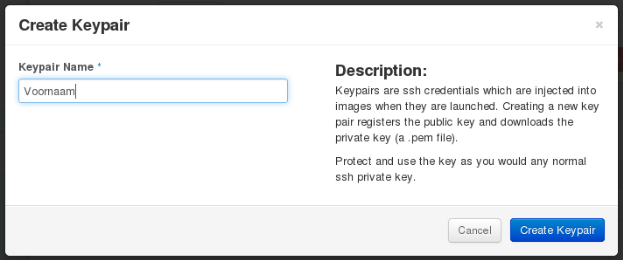
\includegraphics[width=\columnwidth]{images/keypair-2.png}
    \label{fig:graph}
  \end{figure}
  \item Seguidamente se pedir\'a que guarde un archivo \emph{.pem}. Este archivo debe ser guardado en una ubicaci\'on conveniente ya que no ser\'a posible descargarlo de nuevo.
\end{enumerate}

NOTA: Distintos sistemas poseen distintos procedimientos para la conversi\'on del keypair.

\subsection{FreePBX}
NOTA: Todo este proceso debe ser llevado a cabo como administrador. Usar \emph{sudo} luego no va a funcionar. Favor no ignorar esto.

\begin{enumerate}
  \item Ingresar Ubuntu o cambiar a usuario administrador (\emph{root}).
  \begin{figure}[!h]
    \centering
      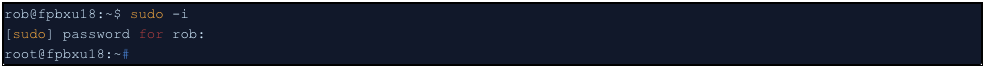
\includegraphics[width=\columnwidth]{images/pbx-1.png}
    \label{fig:graph}
  \end{figure}
  
  \item Habilitar ingresos ssh como administrador.
  \begin{figure}[!h]
    \centering
      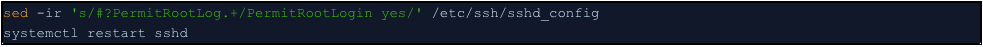
\includegraphics[width=\columnwidth]{images/pbx-2.png}
    \label{fig:graph}
  \end{figure}
  
  \item Actualizar el sistema.
  \begin{figure}[!h]
    \centering
      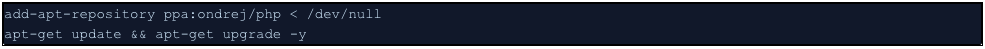
\includegraphics[width=\columnwidth]{images/pbx-3.png}
    \label{fig:graph}
  \end{figure}
  
  \item Instalar dependencias.
  \begin{figure}[!h]
    \centering
      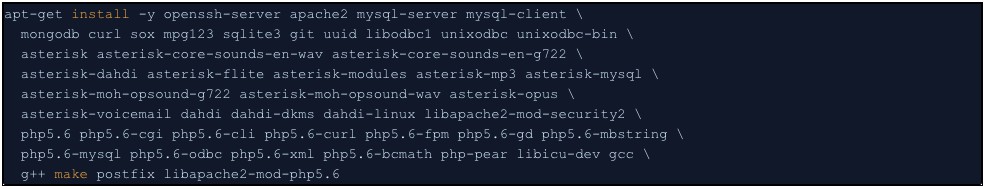
\includegraphics[width=\columnwidth]{images/pbx-4.png}
    \label{fig:graph}
  \end{figure}
  
  \item Instalar NodeJS.
  \begin{figure}[!h]
    \centering
      
\includegraphics[width=\columnwidth]{images/pbx-5.png}
    \label{fig:graph}
  \end{figure}
  
  \item Arreglar los permisos del usuario asterisk
  \begin{figure}[!h]
    \centering
      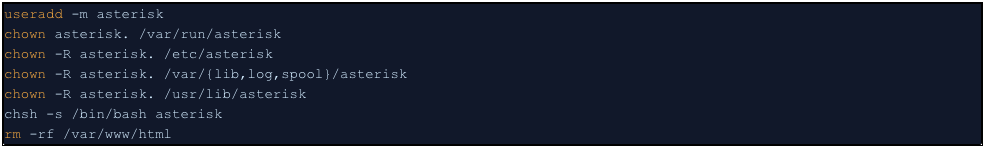
\includegraphics[width=\columnwidth]{images/pbx-6.png}
    \label{fig:graph}
  \end{figure}

  \item Remover ejemplos de archivos config resultantes y arreglar errores
  \begin{figure}[!h]
    \centering
      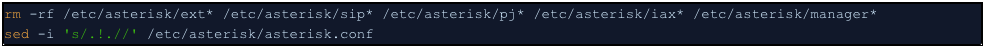
\includegraphics[width=\columnwidth]{images/pbx-7.png}
    \label{fig:graph}
  \end{figure}
  
  \item Actualizar la configuraci\'on de Apache
  \begin{figure}[!h]
    \centering
      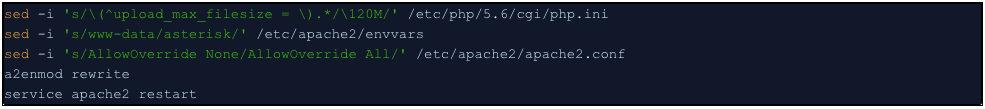
\includegraphics[width=\columnwidth]{images/pbx-8.png}
    \label{fig:graph}
  \end{figure}
  
  \item Arreglar problema de compatibilidad de Pear-GetOpt
  \begin{figure}[!h]
    \centering
      
\includegraphics[width=\columnwidth]{images/pbx-9.png}
    \label{fig:graph}
  \end{figure}
  
  \item Instalar MySQL ODBC Connector
  \begin{figure}[!h]
    \centering
      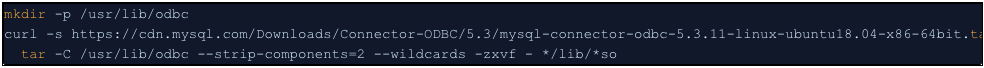
\includegraphics[width=\columnwidth]{images/pbx-10.png}
    \label{fig:graph}
  \end{figure}
  
  \item Configurar el ODBC
  \begin{figure}[!h]
    \centering
      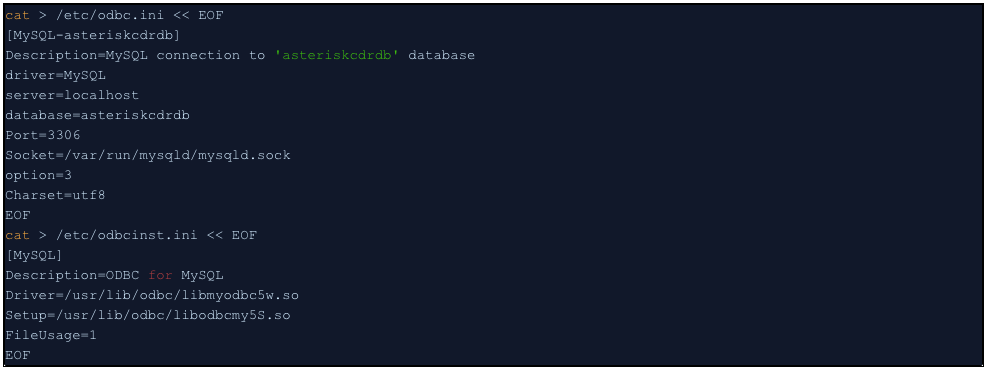
\includegraphics[width=\columnwidth]{images/pbx-11.png}
    \label{fig:graph}
  \end{figure}
  
  \item Descargar e instalar FreePBX 14
  \begin{figure}[!h]
    \centering
      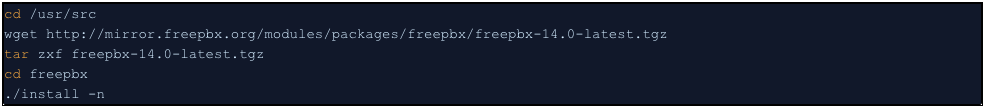
\includegraphics[width=\columnwidth]{images/pbx-12.png}
    \label{fig:graph}
  \end{figure}
\end{enumerate}


\section{Bit\'acora de trabajo}
\subsection{Allan Rojas}
\begin{itemize}
  \item 29-09-2018:
  \begin{itemize}
    \item 3 horas – Buzzer Python
  \end{itemize}
  \item 29-09-2018:
  \begin{itemize}
    \item 4 horas – Database for Node Directory with MariaDB
  \end{itemize}
  \item 30-09-2018:
  \begin{itemize}
    \item 4 horas – Java Audio Listening Programming
  \end{itemize}
  \item 30-09-2018:
  \begin{itemize}
    \item 3 horas – Media Access to Raspberry
  \end{itemize}
  \item 01-10-2018:
  \begin{itemize}
    \item 5 horas – Mac Address Get / Add to Package
  \end{itemize}
  \item 10-10-2018:
  \begin{itemize}
    \item 6 horas – Package Generation and Onion Routing
  \end{itemize}
  \item 19-10-2018:
  \begin{itemize}
    \item 4 horas – Scapy Implementation add to Buzzer
  \end{itemize}
  \item 29-10-2018:
  \begin{itemize}
    \item 6 horas – Scapy Implementation add to Buzzer
  \end{itemize}
\end{itemize}
Total de Horas Trabajadas : 35

\subsection{Sa\'ul Zamora}
\begin{itemize}
  \item 10-11-2018:
  \begin{itemize}
    \item 4 horas - Investigar OpenStack. Tratar de ingresar.
  \end{itemize}
  \item 17-11-2018:
  \begin{itemize}
    \item 1 hora - Creaci\'on de m\'aquina virtual de Ubuntu 18.
    \item 1 hora - Configuraci\'on de VPN en m\'aquina virtual de Ubuntu.
    \item 2 horas - Ingreso a OpenStack dashboard. Primeros intentos de crear instancias.
  \end{itemize}
  \item 18-11-2018:
  \begin{itemize}
    \item 4 horas - Creaci\'on de instancias en OpenStack. Constantes errores. Sin \'exito.
  \end{itemize}
  \item 19-11-2018:
  \begin{itemize}
    \item 2 horas - Creaci\'on de instancias en OpenStack. Constantes errores. Sin \'exito.
  \end{itemize}
  \item 20-11-2018:
  \begin{itemize}
    \item 2 horas - Creaci\'on de instancias en OpenStack. Constantes errores. Sin \'exito.
  \end{itemize}
  \item 23-11-2018:
  \begin{itemize}
    \item 2 horas - Creaci\'on de instancias en OpenStack. Constantes errores. Sin \'exito.
  \end{itemize}
  \item 24-11-2018:
  \begin{itemize}
    \item 3 horas - Instalaci\'on de FreePBX en m\'aquina virtual de Ubuntu.
  \end{itemize}
  \item 25-11-2018:
  \begin{itemize}
    \item 4 horas - Documentaci\'on.
  \end{itemize}
  \item 26-11-2018:
  \begin{itemize}
    \item 4 horas - Documentaci\'on.
  \end{itemize}
  \item 27-11-2018:
  \begin{itemize}
    \item 4 horas - Documentaci\'on.
  \end{itemize}
\end{itemize}
Total de horas trabajadas: 33 horas.

\section{Comentarios finales}
\begin{itemize}
  \item Debido a la falta de configuraciones para el acceso a la VPN no fue posible dar inicio al proyecto desde que fue entregado el enunciado.
  \item Constantes problemas con el funcionamiento de OpenStack hicieron imposible la creaci\'on de instancias de cualquier tipo y por ende la configuraci\'on de cualquier servicio utilizando virtualizaci\'on.
\end{itemize}

\section{Conclusiones}
\begin{itemize}
  \item El uso de virtualizaci\'on es muy \'util en el desarrollo y configuraci\'on de servicios (al igual que el desarrollo de software en general) para la optimizaci\'on de recursos y para invisibilizar las diferencias de hardware en el sistema al usuario final.
  \item 
\end{itemize}

\begin{thebibliography}{9}
  \bibitem{pbx}
  Wiki.freepbx.org. (2018). \emph{Installing FreePBX 14 on Ubuntu 18.04 - FreePBX OpenSource Project - Documentation.}
  [online] Available at: \url{https://wiki.freepbx.org/display/FOP/Installing+FreePBX+14+on+Ubuntu+18.04}

  \bibitem{instances}
  GitHub. (2018). naturalis/openstack-docs.
  [online] Available at: \url{https://github.com/naturalis/openstack-docs/wiki/Howto:-Deploy-a-Windows-image}

  \bibitem{keypairs-windows}
  GitHub. (2018). naturalis/openstack-docs.
  [online] Available at: \url{https://github.com/naturalis/openstack-docs/wiki/Howto:-Creating-and-using-OpenStack-SSH-keypairs-on-Windows}

  \bibitem{keypairs-ubuntu-mac}
  GitHub. (2018). naturalis/openstack-docs.
  [online] Available at: \url{https://github.com/naturalis/openstack-docs/wiki/Howto:-Creating-and-using-OpenStack-SSH-keypairs-on-Linux-and-OSX}

\end{thebibliography}

\end{document}
